
\documentclass[12pt]{article}

% Packages for page layout
\usepackage[margin=1in]{geometry}
\usepackage{fancyhdr}
\usepackage{graphicx}

% Packages for math
\usepackage{amsmath, amsthm, amssymb, amsfonts}

% Packages for graphics
\usepackage{graphicx}
\usepackage{float}

% Header and footer
\pagestyle{fancy}
\fancyhf{}
\rhead{Rex's Trigonometry Problem Set}
\lhead{}
\rfoot{Page \thepage}

% Title page
\title{
    \vspace{2in}
    \textbf{Trigonometry Problem Set}\\
    \vspace{0.1in}
    \large for Class\\
    \vspace{3in}
}
\author{Rex}
\date{}

\begin{document}

\maketitle
\newpage

% Begin enumeration for problems
\begin{enumerate}
    
    
    % Problem 1
    \item \textbf{Evaluate the following expression.}
    \[ \tan(\cos^{-1}(\frac{2}{5})) \]
    
    % Solution
    The exact value of the expression is:
    \[ \frac{\sqrt{21}}{2} \]
    % Space for the solution
    \vspace{45mm}
    % Solution goes here
    % Problem 2
    \item \textbf{Which of the following is equivalent to \( \tan(\theta) \csc(\theta) \sin(\theta) \) for all values of \( \theta \) for which \( \tan(\theta) \csc(\theta) \sin(\theta) \) is defined?}
    
    \begin{itemize}
        \item \( \csc(\theta) \)
        \item \( \sin(\theta) \)
        \item \( \tan(\theta) \)
        \item \( \cot(\theta) \)
    \end{itemize}
    
    % Solution
    The equivalent expression is:
    \[ \tan(\theta) \]
    % Space for the solution
    \vspace{45mm}
    % Solution goes here
   \newpage 
    % Problem 3
    \item \textbf{Simplify the expression \( \sin^{-1}(\tan(\frac{9\pi}{4})) \), where the angle is measured in radians.}
    
    % Solution
    The simplified expression is:
    \[ \frac{\pi}{2} \]
    % Space for the solution
    \vspace{45mm}
    % Solution goes here

    % Problem 4
    \item \textbf{On the domain of \( [-2\pi, 0) \), for what value(s) of \( x \) will \( \sin(-x) = \csc(-x) \)?}
    
    \textit{Enter your answer as an equation, \( x=a \). If there is more than one answer, separate each equation with a comma, \( x=a, x=b \).}
    
    % Solution
    The values for which the equation holds are:
    \[ x = -\frac{3\pi}{2}, x = -\frac{\pi}{2} \]
    % Space for the solution
    \vspace{45mm}
    % Solution goes here
    \newpage
    % Problem 5
    \item \textbf{Solve the following equation for \( \theta \) on the interval \( [0,2\pi) \):}
    \[ 5\sqrt{3} \tan(\theta) - 4 = 1 \]
    
    \textit{List the angles separated by commas if there are multiple answers, e.g. \( \frac{\pi}{3}, \frac{\pi}{2} \).}
    
    % Solution
    The solutions to the equation are:
    \[ \theta = \frac{\pi}{6}, \frac{7\pi}{6} \]
    % Space for the solution
    \vspace{45mm}
    % Solution goes here
    
    % Problem 6
    \item \textbf{Simplify the expression \( \tan(\sin^{-1}(-\frac{12}{37})) \).}
    
    % Solution
    The simplified expression is:
    \[ -\frac{12}{35} \]
    % Space for the solution
    \vspace{45mm}
    % Solution goes here
  \newpage 
    % Problem 7
    
    \item \textbf{Determine a point not in the domain of the function \( f(x) = -\frac{\cot(x)}{4} \) within the interval \( -2\pi < x < 2\pi \).}

    % Graph
    \begin{figure}[h!]
    \centering
    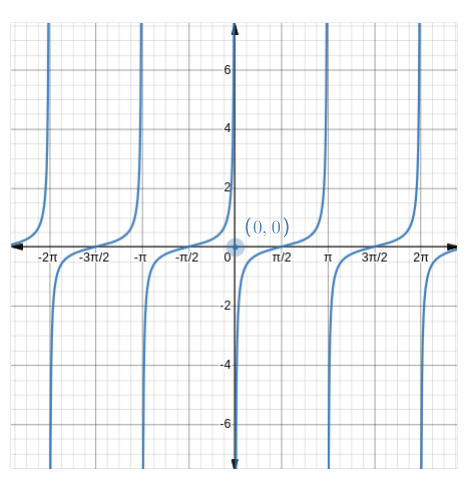
\includegraphics[width=0.75\textwidth]{graph.png} % Replace with the path to your image file
    \caption{Graph of the function \( f(x) = -\frac{\cot(x)}{4} \)}
    \end{figure}

    % Solution
    The function \( f(x) = -\frac{\cot(x)}{4} \) is undefined where \( \cot(x) \) is undefined. The cotangent function is the reciprocal of the tangent function, which is undefined where the tangent function is zero, i.e., at multiples of \( \pi \). Therefore, the points where \( f(x) \) is undefined are at \( x = k\pi \) for any integer \( k \).

    In the interval \( -2\pi < x < 2\pi \), the values for \( k \) that satisfy \( x = k\pi \) are \( k = -1, 0, 1 \). Thus, the points not in the domain are:

    \[ x = -\pi, 0, \pi \]

    However, since the interval is open (does not include the endpoints), we exclude \( x = -2\pi \) and \( x = 2\pi \) from our consideration. Hence, the points not in the domain of \( f(x) \) within the given interval are \( x = -\pi \) and \( x = \pi \).

%   Space for the solution
    \vspace{45mm}
    % Solution goes here
    The points not in the domain of \( f(x) \) are:
    \[ x = -\pi, \pi \]
    % Problem 8
    \item \textbf{Solve for \( \theta \) if \( 16\sin(\theta) + 11 = 27 \) and \( 0 \leq \theta < 2\pi \).}
    
    % Solution
    The solution to the equation is:
    \[ \theta = \frac{\pi}{2} \]
    % Space for the solution
    \vspace{45mm}
    % Solution goes here
    % Problem 9
    \item \textbf{On the graph of \( f(x) = \sec(x) \) and the interval \( [0,2\pi) \), for what value(s) of \( x \) does \( f(x) = -\sqrt{2} \)?}
    
    \textit{Enter your answer as an equation, \( x=a \). If there is more than one answer, separate each equation with a comma, \( x=a, x=b \).}
    
    % Solution
    The values for which the equation holds are:
    \[ x = \frac{3\pi}{4}, x = \frac{5\pi}{4} \]
    % Space for the solution
    \vspace{45mm}
    % Solution goes here
   \newpage 
    % Problem 10
    \item \textbf{Solve the following equation for \( \theta \) on the interval \( [0,360^\circ) \):}
    \[ 2\sec(\theta) - 4 = -2 \]
    
    \textit{Enter your answer as an equation, \( x=a \). If there is more than one answer, separate each equation with a comma, \( x=a, x=b \).}
    
    % Solution
    The solution to the equation is:
    \[ \theta = 0^\circ \]
    % Space for the solution
    \vspace{45mm}
    % Solution goes here
 \end{enumerate}
\end{document}

